\section{Мета практикуму}
Практично ознайомитися із тестами перевірки чисел на простоту, методами генерації ключів для асиметричної криптосистеми типу RSA, протоколом розсилання ключів та безпосередньо реалізувати їх.

\subsection{Постановка задачі та варіант}
\begin{tabularx}{\textwidth}{X|X}
	\textbf{Треба виконати} & \textbf{Зроблено} \\
	Описати побудову алгоритму \checkmark\\
	Порахувати таблицю ймовірностей $P(\textit{M}|\textit{C})$ \checkmark\\
	Показати детермінитичну та стохастичну функції у вигляді таблиць & \checkmark\\
	Порахувати середні витрати для вирішуючих функцій & \checkmark\\
\end{tabularx}



\section{Хід роботи/Опис труднощів}
На початку релазіції практикуму, треба було вибрати генератор псевдовипадкових чисел із попередньої лабораторної роботи та  використати тут. Не довго думаючи, обрав влаштований генератор, що працює на алгоритмі ChaCha12 і дає найкращі результати на тестуванні послідовності. Труднощів із реалізацією самої криптосистеми RSA не було, одразу  функціонал підпису та шифрування розбив на RsaEncryptor, RsaSigner, що спростило подальшу роботу. Також проблем із написанням тесту Міллера-Рабіна, розширеного алгоритму Евкліда не виникало, адже вони уже були написані і відлагоджені у курсі Теоретико-Числових Алгортимів.
Хочу додати, що для генерації простого числа застосовую комбінацію алгоритмів Міллера-Рабіна та пробні ділення (перші 100 простих). Уже для 2048 бітних чисел треба куди більше часу чекати, ніж на менші, але дочекатися можна.


\begin{figure}[h]
			\center{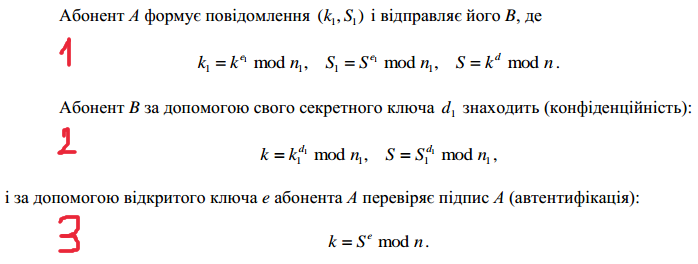
\includegraphics[scale = 0.47]{key_exchange}}
			\caption{Вигляд протоколу.}
			\label{fig:protocole}
		\end{figure}


\section{Результати дослідження}

\subsection{Опис алгоритму}

\subsection{Таблиця ймовірностей}

\subsection{Детерміністична та стохастична матриці}

\subsection{Середні витрати для вирішуючих функцій}

\section{Висновки}
За допомогою реалізації практикуму ''Вивчення криптосистеми RSA та алгоритму електронного
підпису'' дізнався на практиці, як генеруться параметри для асиметричних криптосистем та як реалізовувати їх. 

Рекомендую для алгоритмів знаходження псевдопростих чисел одразу додавати алгоритм пробних ділень. Він значно скоротить час перебору чисел.

		

	




